%% This is an example first chapter.  You should put chapter/appendix that you
%% write into a separate file, and add a line \include{yourfilename} to
%% main.tex, where `yourfilename.tex' is the name of the chapter/appendix file.
%% You can process specific files by typing their names in at the 
%% \files=
%% prompt when you run the file main.tex through LaTeX.
\chapter{Codeable Objects}

\begin{center}
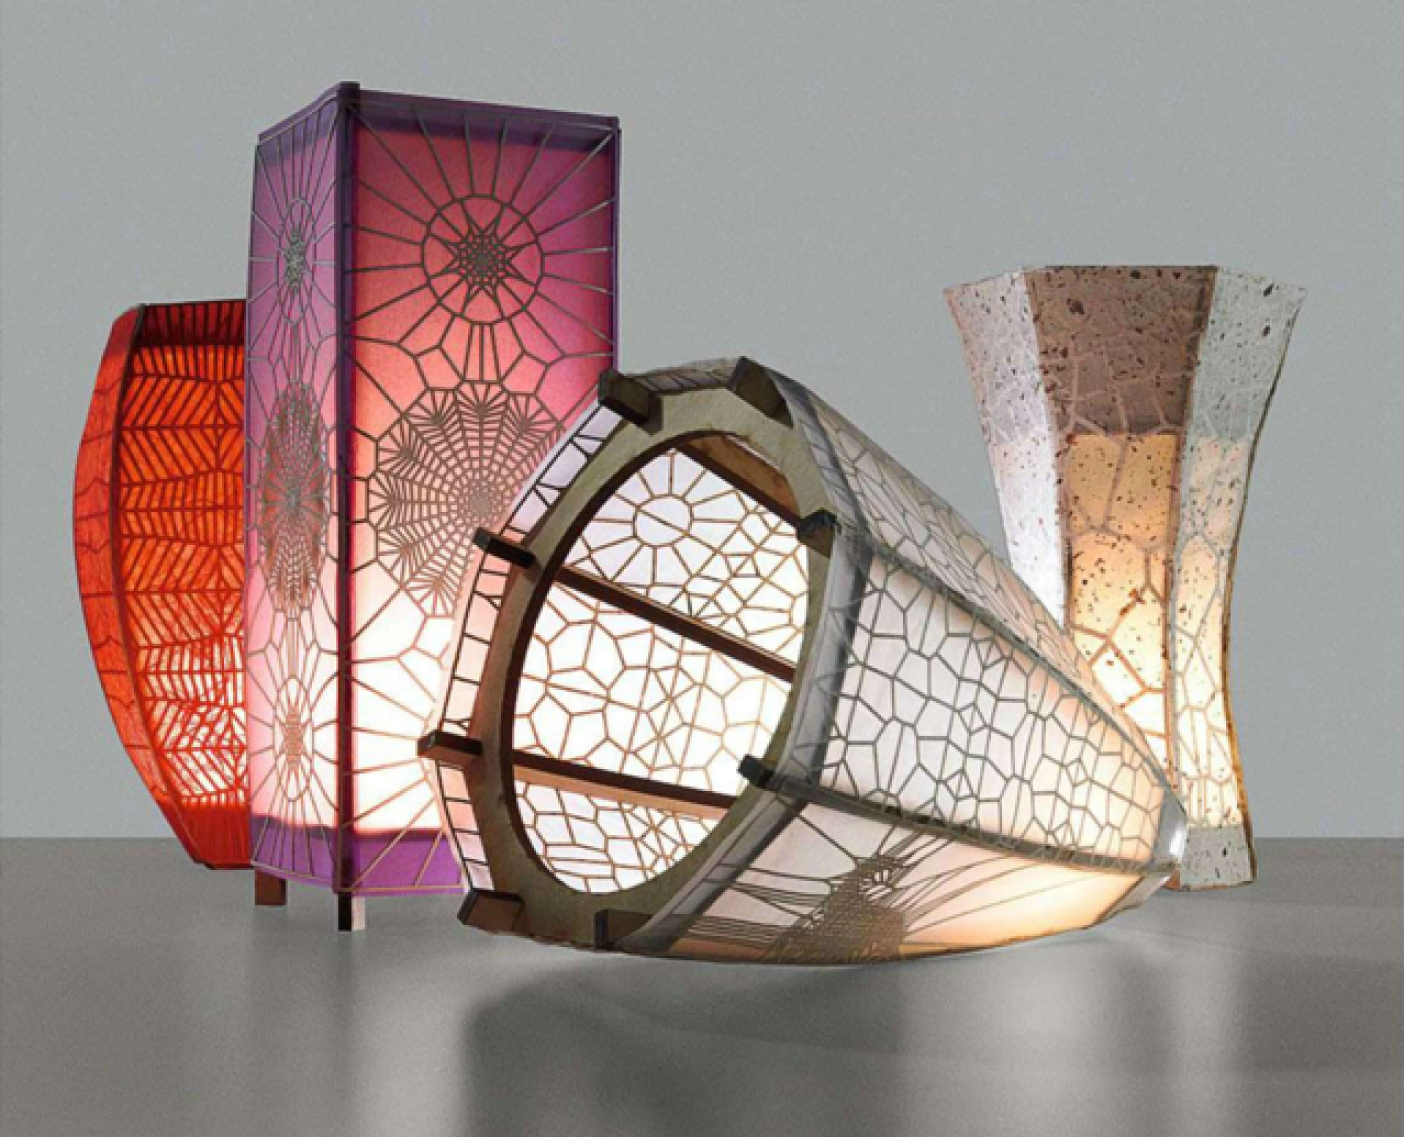
\includegraphics[width=6.5in]{images/finished_lamps.png}
\end{center}

Codeable Objects is computational design tool that allowed people to design a laser cut lamp. The choice of a lamp allowed for a relatively broad design space wherein aesthetics were a primary consideration, while still retaining the qualities of functionality and utility in the finished product.  Lamps possess an established function, but offer a great deal of flexibility and personal freedom in the aesthetics and form. In addition, there is an established history of creating DIY lamps via digital fabrication. The Instructables community tutorial website has an entire section devoted to DIY lamps, and many examples of patterns that use a laser cutter for fabrication. 
\begin{center}
\begin{figure}[h!]
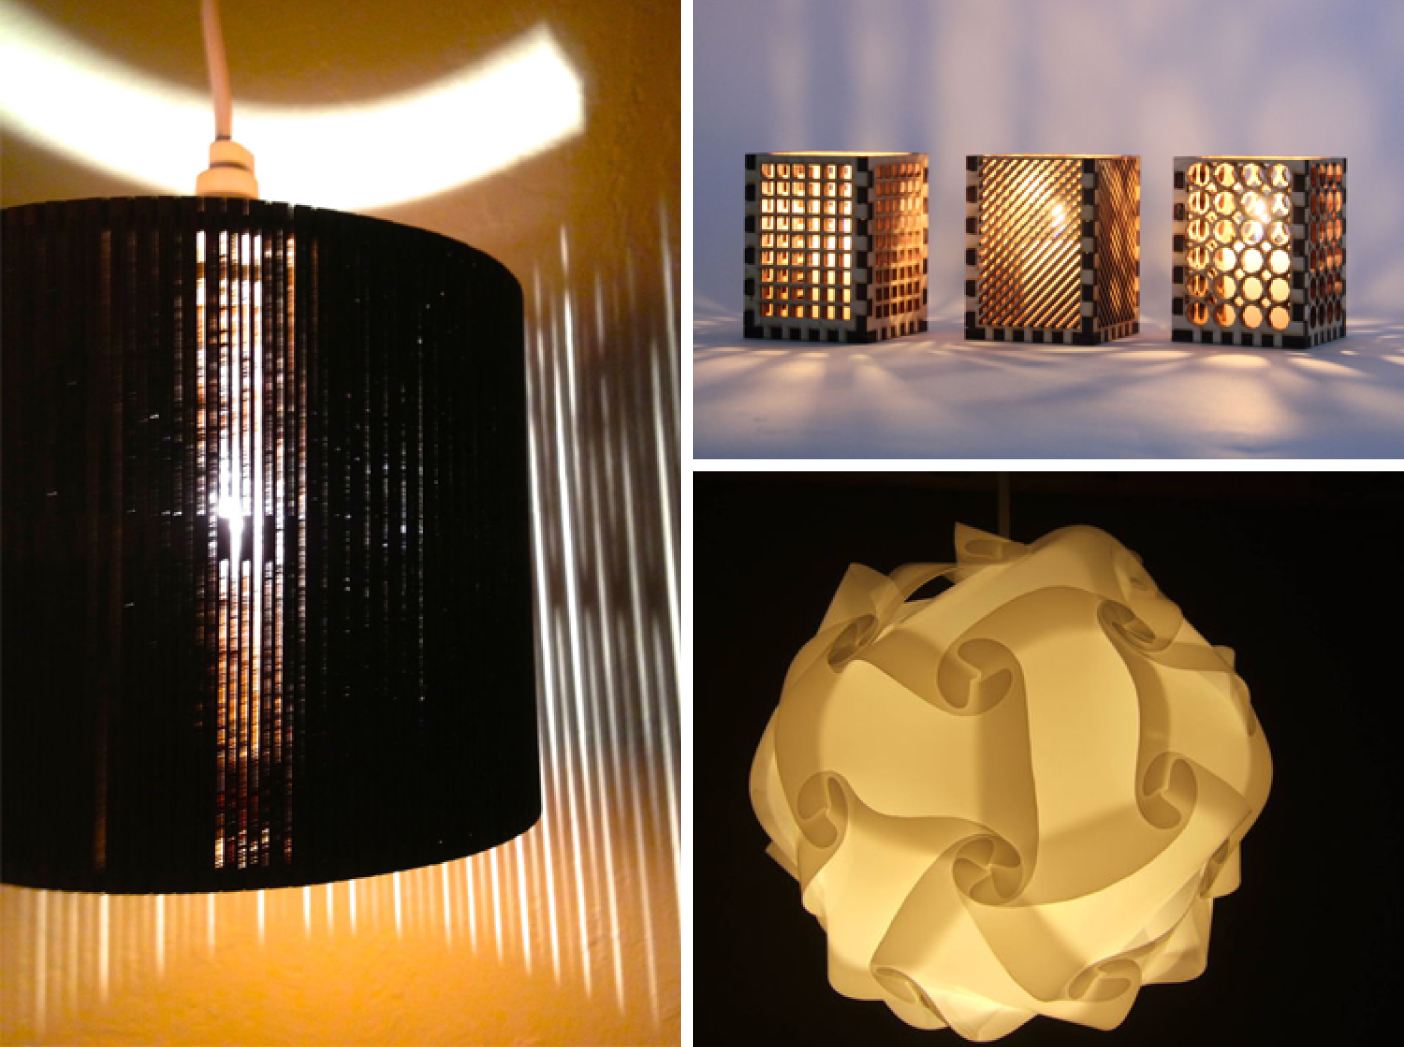
\includegraphics[width=6.5in]{images/instructables_lamps.png}
\caption{a selection of laser cut lamps from Instructables}
\end{figure}
\end{center}
\section{Motivation}
One of the restrictions of many of these examples is that they require the person making the lamp to directly emulate the design provided by the creator of the tutorial. If the person wishes to deviate from the original design, they  need to use a CAD tool like Adobe Illustrator or Solid Works\cite{instructables_lamp_1}. As mentioned in Section \ref{sec:professional_computational_design_tools}, professional CAD tools like Solid Works are often difficult to access and use for casual practitioners. In addition, during my personal experience in using a non-parametric tool like illustrator to design, I often found I had to resort to fabricating numerous sample pieces of in order to ensure the joints and form would function correctly in the final piece. If I made a mistake, or decided I wanted to modify the design, I lost time and materials in the fabricating process, and had to endure the tedious process of adjusting correcting each individual part. 
\begin{center}
\begin{figure}[h!]
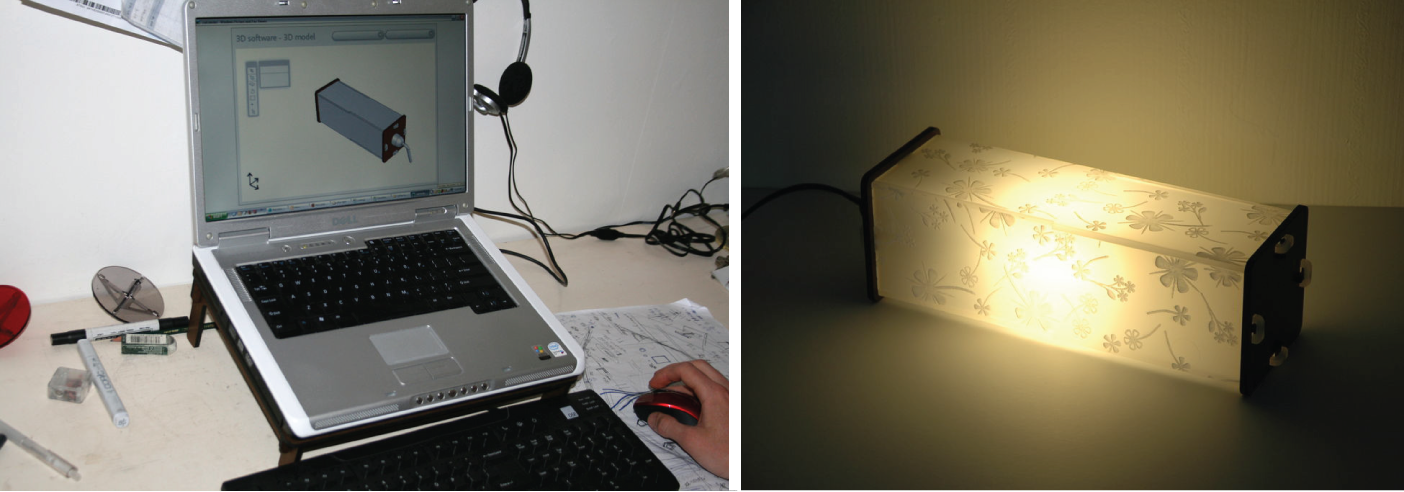
\includegraphics[width=6.5in]{images/solidworks_lamp.png}
\caption{Instructables lamp tutorial with SolidWorks design process}
\end{figure}
\end{center}
One of the most frequent applications of a laser cutter is to create 3D forms by assembling 2D press fit pieces in a frame-like structure. I found that when creating 3D forms that were curved, it was extremely challenging in traditional 2D CAD software to correctly size and design parts which would fit the faces of the form. This was particularly relevant to lamp design, wherein it was necessary to create shades to diffuse the light. The shades also provided an excellent space for incorporating styles and patterns into the lamp. The combined tasks of simplified design and customization, parametric manipulation, and the calculation and conversion of a 3D form to 2D parts indicated that computational design would be a good match for the task of designing and fabricating a laser cut lamp. 
	
\section{Tool Description and workflow}
The objective of the first version of Codeable Objects was simple: to create a tool that allowed to design a custom lamp by describing the form and the pattern of the shades, which they could then fabricate and assemble. The lamp itself was comprised of 4 basic parts, a wooden press fit frame, a set of vellum pieces that fit over the frame to act as a shade,a set of cardstock pieces with a pattern that fit over the shades, and a commercial made light fixture that fit into the frame (see figure: \ref{fig:lamp_parts}.)
\begin{center}
\begin{figure}[h!]
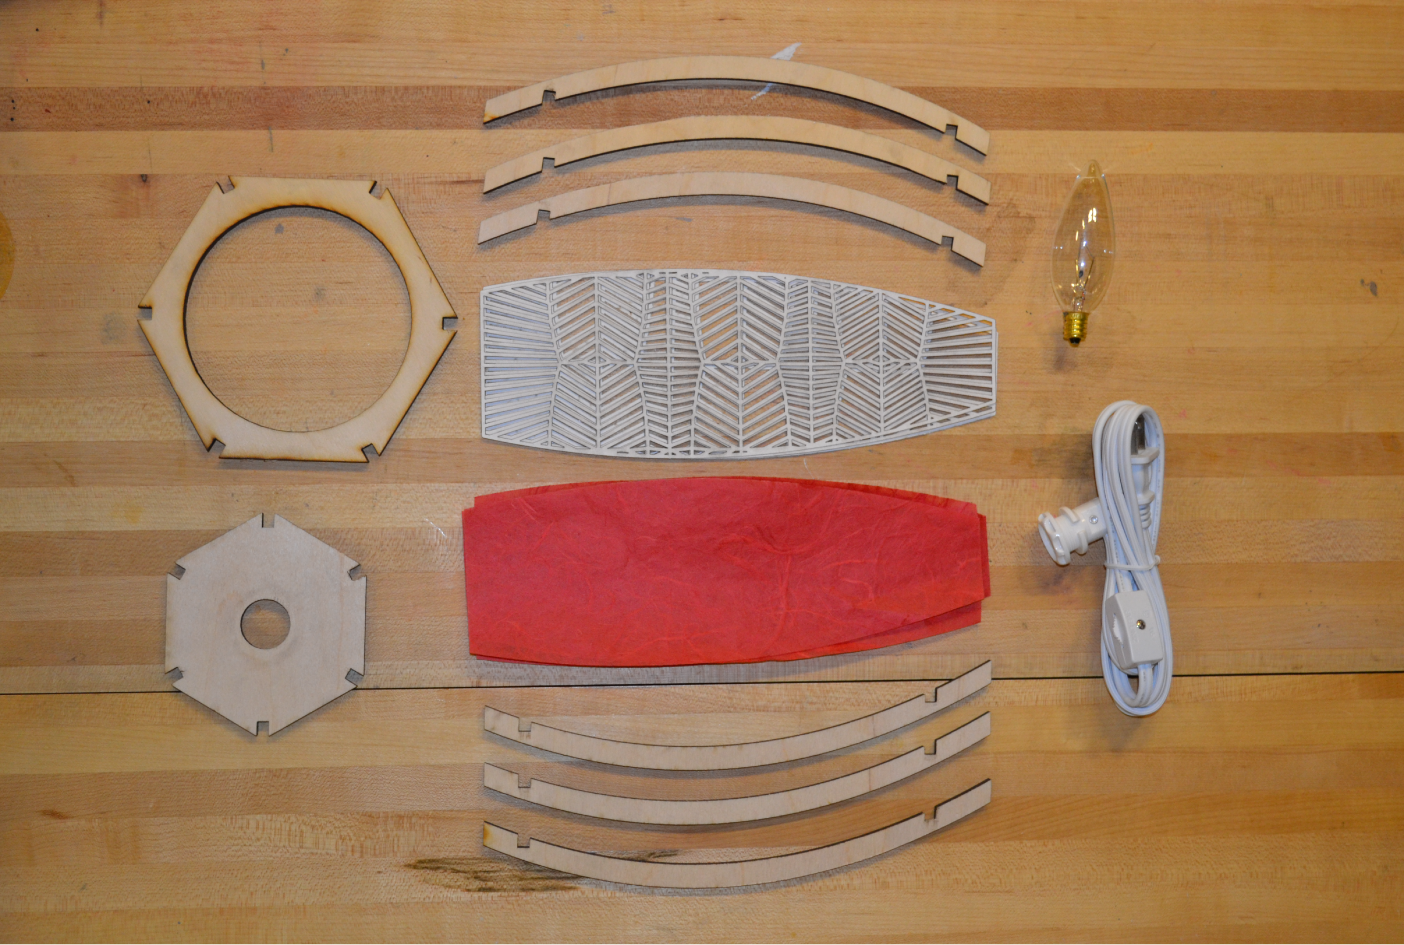
\includegraphics[width=6.5in]{images/parts.png}
\caption{the individual parts of a lamp}
\label{fig:lamp_parts}
\end{figure}
\end{center}
Codeable Objects was developed as a programing library for Processing and contained a set of pre-defined programing methods that allow the user to describe the lamp, and define the tool paths for all three materials. The first version of the library was somewhat rough. All design took place via textual programing, and keyboard commands. Within the Processing IDE one imports and initialize the controller class of the library, and uses it to call four main functions that determine the height, top width, middle width and bottom width of the lamp. These 4 parameters are used to determine the form of the lamp, by generating the equation of a parabola with 3 intersection points. By rotating this parabola round the y-axis, it was possible to generate a closed 3-dimensional ellipsoid form.  The library also provided access to an additional set of methods that control over a number of other parameters in describing the form of the lamp, including the number of sides, the resolution of the curve and the position of the internal structural supports. To facilitate the construction process, notches are automatically generated in all of the individual parts to allow the form of the lamp to be press-fit together. The inclusion of this feature gives the user freedom to customize the shape of their lamp, without having to worry about the mechanics of construction. The library determines the correct position of the notches by calculating appropriate angle for each individual notch and determining the correct edge of intersection for each tool path based on this angle.  

 Codeable Objects also includes a second set of programing methods that allow users to describe the  decorative components of the lamp by specifying coordinates in polar or Cartesian space. Upon compilation, the coordinates are used by the application to calculate a design using a Voronoi diagram. A Voronoi diagram is a geometric subdivision of space that generates a quadrants based on a given point set according to the equidistant boundaries between all the points \cite{deBerg}. When the diagram is calculated, each segment is checked for intersection or containment with the polygon. Segments with both endpoints within the polygon are preserved unchanged, while segments with only one endpoint inside the diagram are clipped at the appropriate edge of intersection, by checking their angle against the angle of the points of the edges of the boundary. Segments which have both points outside of the polygon are checked for intersection using the segment intersection algorithm and either clipped according to their intersection points or removed altogether if they lack an intersection (fig: \ref{fig:voronoi_clipped}).
 \begin{wrapfigure}{r}{0.5\textwidth}
  \vspace{-20pt}
 \begin{center}
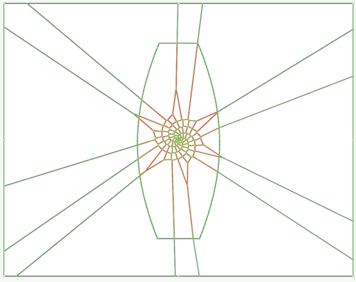
\includegraphics[scale=0.5]{images/voronoi_clipped.png}
\end{center}
\caption{Algorithim for constraining the voronoi diagram within the shade}
\label{fig:voronoi_clipped}
  \vspace{-10pt}
\end{wrapfigure}
  
Once the code is compiled, a graphic preview is displayed. For the pilot version, users could use key-commands to toggle between a view of the form of the 3D form of lamp, the voronoi-diagram pattern, and a 2D preview of the press fit parts (fig:\ref{fig:codeable_objects_v1}.) A final key-command allowed for the resultant design files to be exported as three separate pdfs, containing the paths for the press-fit frame, the shades, and the pattern files. 

\begin{center}
\begin{figure}[h!]
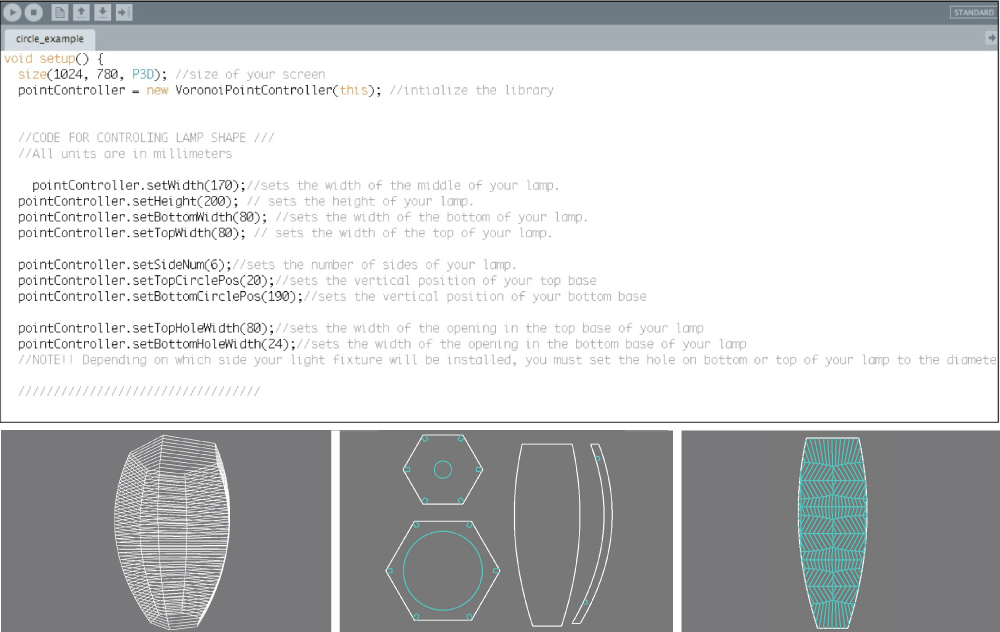
\includegraphics[width=6.5in]{images/codeable_objects_v1.jpg}
\caption{The first version of Codeable Objects, with only text-based interaction}
\label{fig:codeable_objects_v1}
\end{figure}
\end{center}
		
\section{Evaluation}
Using this basic pilot library, the first evaluation of Codeable Objects was conducted with a group of nine graduate students, ranging in age from 24-34, who engaged in a six-hour workshop. Five participants were women.  According to self-reported pre-survey data, all but one of the participants were intermediate to experienced programmers. Five of the nine had previous experience with Processing. In contrast, participants indicated they had little or no prior experience in design.  What experience they had was primarily gained in high school art classes and college elective courses. 
During the workshop, each participants engaged in the design and fabrication of a lamp. Participants received programing instruction in the use of Codeable Objects and a basic explanation of the principles behind the geometry of the lamp. The pilot version of Codeable Objects was packaged with a set of example programs that contained the basic code for initializing the library and defining the parameters of the lamp, a long with a variety of point generation methods. Examples included algorithms to generate spirals, circles and sine and cosine wave distributions of points. Participants were also provided with access to materials, and received training in the use of the laser cutter. Participants were given approximately four hours to design the structure and ornamentation of their lamp, followed by instruction on and access to the laser cutter. After cutting, participants were provided instructions about how to assemble their lamps. 

\begin{center}
\begin{figure}[h!]
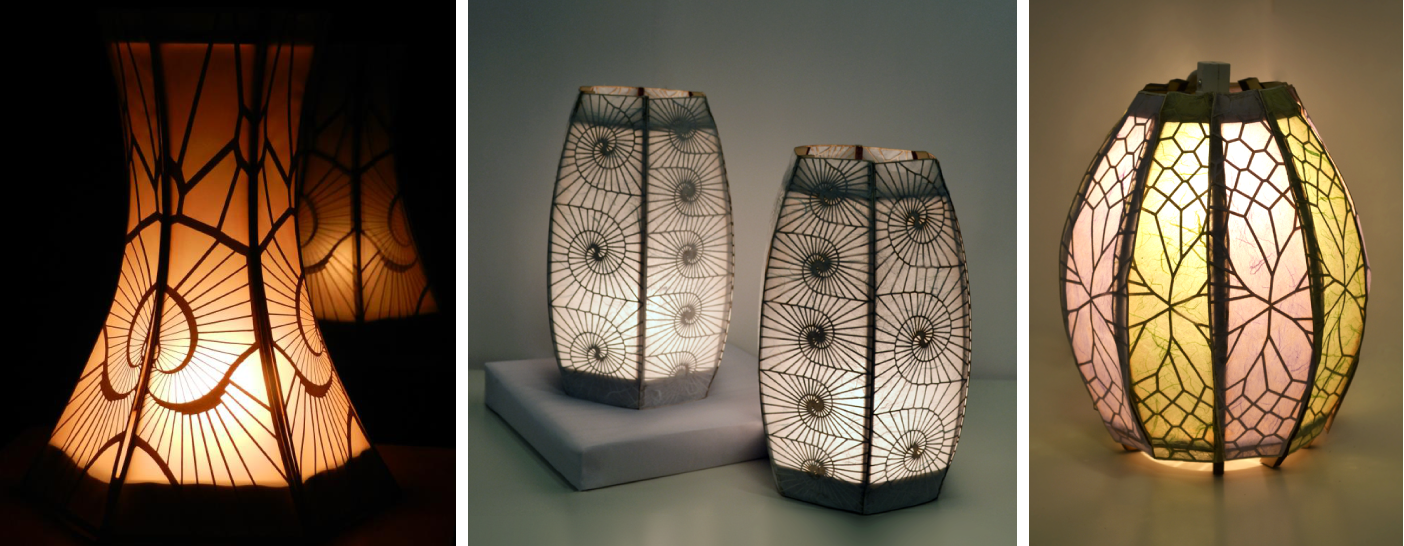
\includegraphics[width=6.5in]{images/finished_lamps2.png}
\caption{Several of the finished lamps from the first workshop}
\label{fig:finished_lamps}
\end{figure}
\end{center}

\section{ Results}
All but one of the participants in the Lamp workshop successfully completed their lamp. The one exception was a user who wished to incorporate a specialized light fixture into their piece, but unfortunately damaged her parts while waiting for the fixture to arrive. Participants with little or no prior programing experience primarily relied upon tweaking or remixing the example programs to design the form and pattern of their lamp, whereas those more experienced in programing experimented extensively with the library to produce a wide range of forms and patterns. One participant wrote a program that decomposed a black and white image into a point cloud and used that as the basis for her pattern. Another participant wrote a program that used a Gaussian distribution of points to achieve the gradual variation he desired in his final pattern. 

 The physical assembly process required additional time beyond the duration of the workshop for most participants. This can partially be attributed to the bottleneck on the laser cutter, however the design and crafting components of the project took longer than expected. Despite this, all the participants returned after the workshop to complete their projects, and each participants indicated on the survey that they were able to complete a finished product to their satisfaction. The physical objects produced were both attractive and functional; participants displayed their lamps in their offices and homes after completion. One participant returned several days later to build a second lamp so that he would have a matching set for his bedside tables (figure:\ref{fig:finished_lamps}.)		
		
		
\section{Discussion}

%The most evident success of the pilot version of Codeable objects was the high rate of project completion. This success rate was closely connected to the ability of the library to correctly constrain the design parameters of the lamp. Although participants at times had to re-fabricate parts due to incorrect settings on the laser cutter or variations in the physical materials, at no point did a participant have to re-fabricate their piece due to errors in the design itself. Once fabricated, all participants pieces fit together correctly. This success came at the cost however, of significant design limitations. Participants who wished to modify the form to have more than one curve, or create patterns that went beyond the restrictions of the Voronoi diagram had to resort to post-processing their design files with a different CAD tool. In general, the %

Because of their prior expertise, the experiences of the majority of the participants in the first study are not indicative of the feasibility of Codeable Objects for novice programmers. Their experiences provide valuable contrast to the experience of the novice coders in the successive workshops however, and provide important information about the usability and workflow of the software. Despite their experience in programing however, the experienced programmers in the lamp workshop exhibited limited knowledge of computational design prior to the start of the workshop. When asked in the pre-workshop surveys how they thought programing, design and craft could be combined, the general response was either uncertain, or as method to create dynamic interactivity, rather than a tool for the design of form and pattern:

\textit{``You can combine software and hardware and make craft more dynamic (e.g. sensors). [Lamp Participant pre 1]}

\textit{``[Programing] gives [you] the ability to make something dynamic. [Lamp Participant pre 3]}

Following the workshop, the participants were generally pleased with the creative affordances of the tool, and described how the software enabled them to expand their programing abilities to the realm of art and craft with greater success: 

\textit{``I think programming makes designing more accessible because you don't have to be able to draw or paint. 
[Lamp participant post 4] }

\textit{``I love the idea of being able to combine my interest in programming for creative expressions. 
[Lamp participant post 6]}

There was also an awareness among several participants about the practical benefits of combining computational design and digital fabrication:

\textit{``I understand now how programming can be used for quick prototyping and mockups that can be used to inform final design decisions. This is easy [and] helpful when using physical materials where mistakes can be costly. 
[Lamp participant post 2]}

\textit{``Using programming in the design process adds some exciting and unique capabilities over traditional design and crafting, including mixing in different algorithm and ideas from other existing software, and rapid prototyping of complex designs."[Lamp participant post 6]}

From these responses, it is apparent that even among experienced programmers, algorithmic craft has the potential to expand people's understanding of the applications of programming and motivate them to apply computation to other forms of production and expression. There were also elements of the process and tool that were problematic for the participants. It became immediately clear during the workshop that textual programing was not the optimal method of modifying the form of the lamp. Many of the participants became frustrated about having to set the parameters and then wait for the compilation process to complete before they could view the resulting form. This issue was addressed partly in subsequent versions of the tool by replacing the textual parameters with a set of sliders in the compiled application, which would adjust the form in real time, across each of the views (figure: \ref{fig:slider_interface}.)
\begin{center}
\begin{figure}[h!]
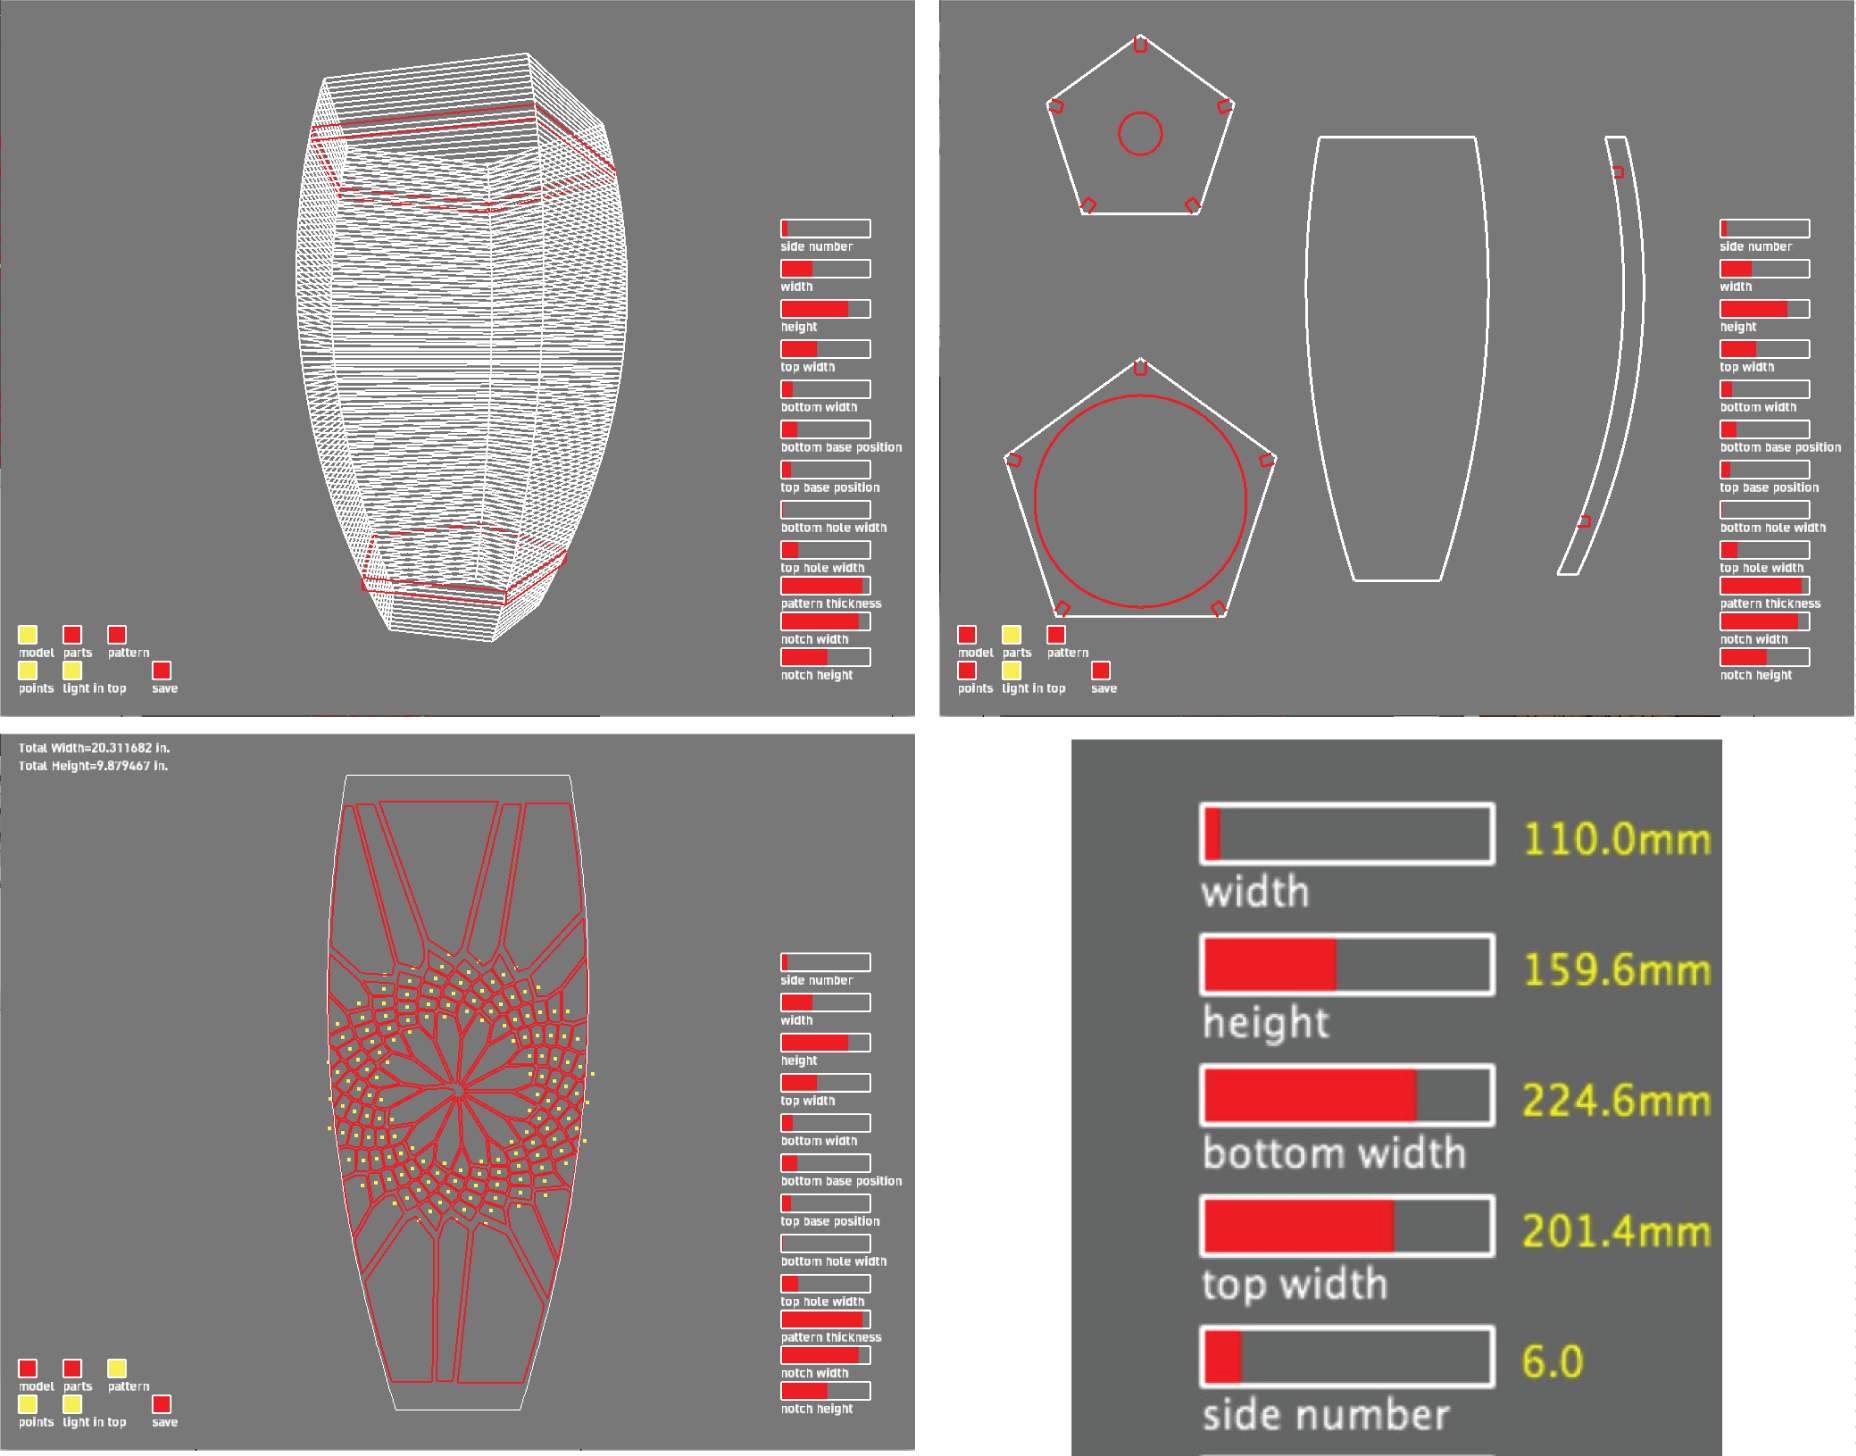
\includegraphics[width=6.5in]{images/slider_interface.png}
\caption{Revised graphic view with sliders}
\label{fig:slider_interface}
\end{figure}
\end{center}

The textual programing method proved to be useful in the context of the point specification for the pattern. The simple method of specifying points in a programing context, allowed for the wide degree of variation and approaches in the resulting designs. If the tool had relied on a more standard set of graphical user interface(UI) components, like sliders to control the point generation, it is doubtful that the same range and creativity could have been achieved. On the other hand, it was clear that the less experienced programmers had more difficulty deliberately designing the patterns of their lamps, and relied primarily on adjusting and remixing existing examples. 

Several participants also put forth detailed critiques of the programming process, which brought into focus concerns about the practice of computational design itself. One participant reacted against defining the generative qualities of the Voronoi diagram patterns as a design method:

 \textit{`"Changing the parameters didn't always generate the pattern you have in mind. It was more like generating a few semi-random patterns and you choose one that looks good. It is rather a trying-and-choosing rather than designing /making something you planned to have. I think "design" involves "intention" and "planning." Programming, crafting, and design should be combined in the way that entails prior planning and intentions as opposed to cutting together the semi-random choices, which could be good but I wouldn't call that design. [Lamp participant post 6]"}
 
This comment addresses the concern that the attributes of randomness and generativity do not automatically lead to optimal or good design decisions. Some deciding factor has to play a role in the process, but the designer�s role in the deciding process is often ambiguous. This criticism touches on a core debate about the role of conscious design and the restriction of intuitive creativity in computational practices overall, however it is particularly relevant to computational design. The emergence of comments like this are encouraging, because they reflect the engagement of the participants, not just with the task at hand, but in a critical evaluation of the  creative implications of this form of creation. This comment however also highlights a key restriction of Codeable Objects. While it is ambiguous to the extent at which adjusting the parameters and input values to a system constitutes design, the task of defining the algorithms which shape the system itself are decidedly a form of design. With Codeable Objects however, the user is unable to modify the core algorithms which define the range of forms and patterns that are possible, unless they alter the source code of the library itself. When evaluated as a tool for algorithmic craft, Codeable Objects could have done a better job of supporting some of the deeper components of computational design, in particular, the algorithmic abstraction of personal styles and aesthetics. The stylistic limitations contained in the tool most likely contributed to the high success rate in project completion, and the general attractiveness of the resulting projects, but the experience of the workshop, provided the motivation for future tools to have better balance of stylistic and computational openness and accessibility for new programmers. 

One other defining component of the Codeable Objects pilot workshop was the stark contrast between the nature of the challenges in the computational design and digital fabrication components and the crafting component. The difficulties people experienced while designing and fabricating their projects were often discrete, for example correcting for mathematical error in coordinate placement, or having the incorrect setting on the laser cutter. More complex problems sometimes arose in these contexts as well, such as confusing on the principles behind some of the more complex point generation algorithms, or the programming aspects in general, however they were seemingly aspects that could be addressed through verbal instruction and explanation. The challenges encountered in the crafting session were of a different quality, concerning the best techniques for assembling the parts so that the resulting product maintained an attractive appearance. Most participants were surprised at the amount of time required to complete the physical assembly, and were often frustrated when variations in the crafting process violated the precision and perfection of the digital design, and laser cut parts. Some of the frustrations in the physical construction process were addressed in subsequent workshops by creating a paper variation of the lamp that was faster and easier to assemble and required no gluing (figure: \ref{fig:paper_lamp}.) In addition, a feature was added to the software which to report the approximate material size required for a design, so that users could ensure their would fit on the bed of the laser cutter. 
\begin{center}
\begin{figure}[h!]
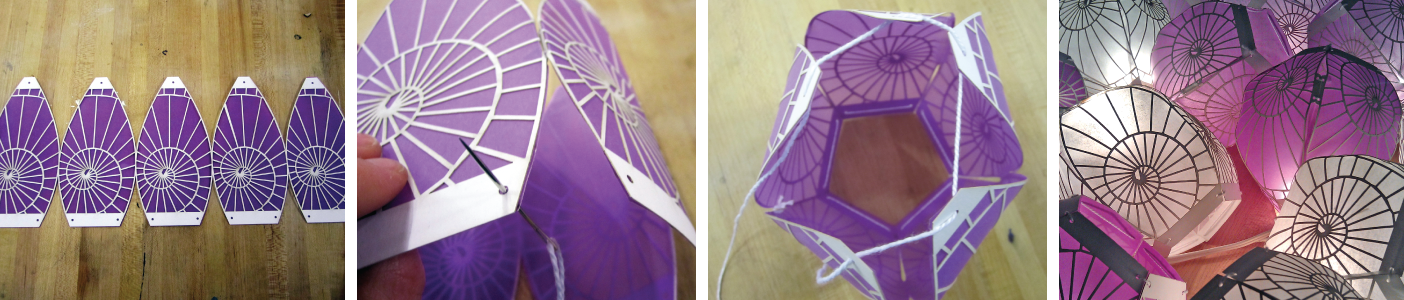
\includegraphics[width=6.5in]{images/paper_lamps.png}
\caption{The revised paper lamps}
\label{fig:paper_lamp}
\end{figure}
\end{center}
Although there is often an opportunity to improve a user's experience through improvements in the interface and artifact design, in craft, it is both impossible and undesirable to eliminate the properties of material variation, and the benefits of practice and experience. Many of the difficulties workshop participants experienced in the crafting process therefore do not reflect a failure in the tools, but rather challenges that are intrinsic to crafting, and best addressed through practice and familiarity with the materials. In this way, craft practice differs from computational practice. While approaches benefit from experience and practice, the approaches for solving problems differ significantly in programing and hand crafting. Programming often requires an analytical approach with an emphasis on consistency and regularity, whereas crafting requires a more intuitive process of responding and adjusting one's technique while in direct contact with the materials. An interesting question is then, how then, can algorithmic tools be presented in a manner that accustom users to operating in both discreet and intuitive modes of problem solving, and furthermore how can these two modes of working inform both craft and computational approaches simultaneously?